\section{Process Discovery}
\subsection{Alpha Miner}
\subsubsection{Exercise 1}
Given the following event log:
\[L_1 = [\langle a,b,c,d \rangle^3, \langle a,c,b,d \rangle^2, \langle a,e,d \rangle^1]\]
build the process model using the Alpha Miner algorithm.
\paragraph{Solution}
\begin{enumerate}
    \item 
\end{enumerate}

\subsubsection{Exercise 2}
Given the following event log:
\[L = \left[ \langle a,b,c,d,e,f,b,d,c,e,g \rangle, \langle a,b,d,c,e,g \rangle^2, \langle a,b,c,d,e,f,b,c,d,e,f,b,d,c,e,g \rangle\right]\]
Use the Alpha Miner algorithm to discover a Petri net from the event log.
\paragraph{Solution:}
\begin{enumerate}
    \item First, we need to compute the footprint matrix:
    \begin{table}[H]
    \centering
    \begin{tabular}{c|ccccccc}
        & A & B & C & D & E & F & G \\
        \hline
        A & $\#$ & $\rightarrow$ & $\#$ & $\#$ & $\#$ & $\#$ & $\#$ \\
        B &  & $\#$ & $\rightarrow$ & $\rightarrow$ & $\#$ & $\leftarrow$ & $\#$ \\
        C &  &  & $\#$ & $||$ & $\rightarrow$ & $\#$ & $\#$ \\
        D &  &  &  & $\#$ & $\rightarrow$ & $\#$ & $\#$ \\
        E &  &  &  &  & $\#$ & $\rightarrow$ & $\rightarrow$ \\
        F &  &  &  &  &  & $\#$ & $\#$ \\
        G &  &  &  &  &  &  & $\#$ \\
    \end{tabular}
    \caption{Footprint Matrix for the Event Log \(L\)}
\end{table}
    \item Next, we identify the sets of all transitions $T_L$, the set of start activities $T_I$ and the set of end activities $T_O$:
    \begin{itemize}
        \item $T_L = \{a,b,c,d,e,f,g\}$
        \item $T_I = \{a\}$
        \item $T_O = \{g\}$
    \end{itemize}
    \item Then, we identify the pairs of sets of transitions that satisfy the Alpha Miner conditions.
    To find the first pairs, we look for causality relations in the footprint matrix:
    \[\{
        (\{a\}, \{b\}),\ 
        (\{b\}, \{c\}),\ 
        (\{b\}, \{d\}),\ 
        (\{f\}, \{b\}),\ 
        (\{c\}, \{e\}),\
        (\{d\}, \{e\}),\
        (\{e\}, \{f\}),
        (\{e\}, \{g\})
    \}
    \]
    \item We can then group these pairs into maximal sets:
    \[\{
        (\{a,f\}, \{b\}),\ 
        (\{e\}, \{f,g\}),\
    \}
    \]
    And we can remove the non-maximal sets that composed them:
    \[\{
        (\{a\}, \{b\}),\
        (\{f\}, \{b\}),\
        (\{e\}, \{f\}),\
        (\{e\}, \{g\})
    \}
    \]
    \item Finally, we can construct the Workflow net, using one place for each of the identified pairs, and connecting them according to the causality relations:
    \begin{figure}[H]
        \centering
        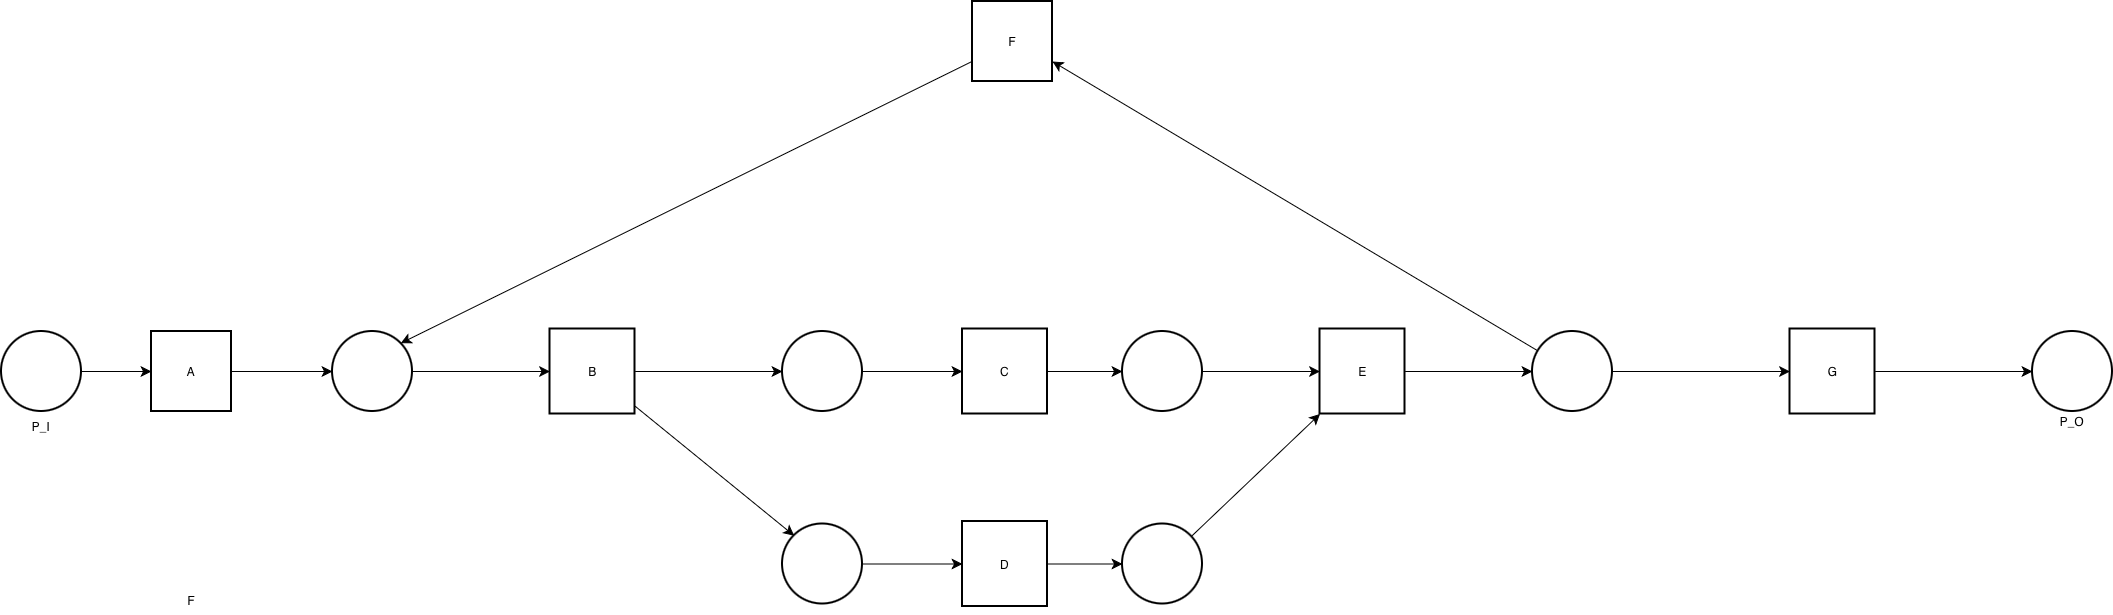
\includegraphics[width=0.7\textwidth]{images/exercises/alpha_miner.png}
        \caption{Petri Net Discovered using the Alpha Miner}
    \end{figure}
\end{enumerate}
\subsubsection{Exercise 3}
Given the following event log:
\[L_4 = [\langle a,c,d \rangle^45, \langle b,c,d \rangle^42, \langle a,c,e \rangle^38, \langle b,c,e \rangle^22]\]
build the process model using the Alpha Miner algorithm.
\paragraph{Solution}
\begin{enumerate}
    \item 
\end{enumerate}